\documentclass[tikz]{standalone}

\usepackage{fontspec}

\usetikzlibrary{arrows}
\usetikzlibrary{calc}
\usetikzlibrary{decorations.pathreplacing}
\usetikzlibrary{positioning}
\usetikzlibrary{matrix}

\usepackage{fontspec}

\begin{document}

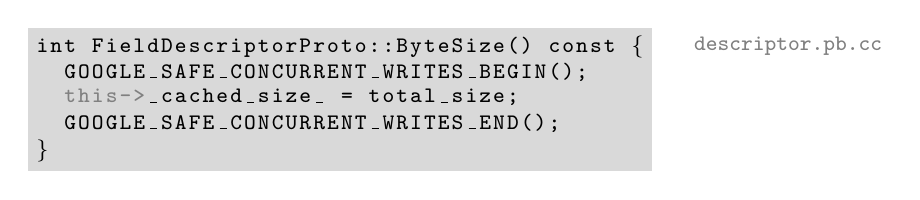
\begin{tikzpicture}
  [node distance=5mm, >=stealth',
  every node/.style={font=\footnotesize},
  every matrix/.style={fill=black!15, inner sep=1mm, row sep=0.5mm,
                        matrix of nodes, nodes in empty cells,
                        minimum height=0.5em, minimum width=.5em,
                        nodes={anchor=base, inner sep=0, font=\ttfamily\footnotesize}}]

  \matrix (snippet) {
i & n & t &   & F & i & e & l & d & D & e & s & c & r & i & p & t & o & r & P & r & o & t & o & : & : & B & y & t & e & S & i & z & e & ( & ) &   & c & o & n & s & t &   & \{ \\
  &   & G & O & O & G & L & E & \_ & S & A & F & E & \_ & C & O & N & C & U & R & R & E & N & T & \_ & W & R & I & T & E & S & \_ & B & E & G & I & N & ( & ) & ; &   &   &   &   \\
  &   & |[black!50]|t & |[black!50]|h & |[black!50]|i & |[black!50]|s & |[black!50]|- & |[black!50]|> & \_ & c & a & c & h & e & d & \_ & s & i & z & e & \_ &   & = &   & t & o & t & a & l & \_ & s & i & z & e & ; &   &   &   &   &   &   &   &   &   \\
  &   & G & O & O & G & L & E & \_ & S & A & F & E & \_ & C & O & N & C & U & R & R & E & N & T & \_ & W & R & I & T & E & S & \_ & E & N & D & ( & ) & ; &   &   &   &   &   &   \\
\} &   &   &   &   &   &   &   &   &   &   &   &   &   &   &   &   &   &   &   &   &   &   &   &   &   &   &   &   &   &   &   &   &   &   &   &   &   &   &   &   &   &   &   \\
  };

  \node [above, anchor=west, black!50, xshift=0.5cm]
        at (snippet-1-44.east)
        {\texttt{descriptor.pb.cc}};
\end{tikzpicture}

\end{document}
